% !TEX root = MAIN.tex
\chapter{Software Development Plan}

% a. The software development life cycle shall be defined or referenced in the software product assurance plan.
% b. The following characteristics of the software life cycle shall be defined:
% 1. phases;
% 2. input and output of each phase;
% 3. status of completion of phase output;
% 4. milestones;
% 5. dependencies;
% 6. responsibilities;
% 7. role of the customer at each milestone review, in conformance with ECSS‐M‐ST‐10 and ECSS‐M‐ST‐10‐01.
% EXPECTED OUTPUT: Software product assurance plan [PAF, SPAP; SRR, PDR].
%
% 6.3.4.5
% a. Use of low‐level programming languages shall be justified.
% EXPECTED OUTPUT: Software development plan

\label{chapter:software_development}
This Chapter contains the Software Development Plan (SDP) for the development of the FAQAS framework. Its purpose is to describe the general management and development approaches used in the production of the FAQAS framework.

\section{Software Project Management Approach}

SnT will be responsible for the coordination and management of the project. Figure~\ref{fig:reporting_lines} presents the project organization describing the project office and the Work Package (WP, task leaders). The project communication and reporting lines follow the structure in Figure~\ref{fig:reporting_lines}.

\begin{figure}[H]
\caption{Project organization.}
\label{fig:reporting_lines}
\centering
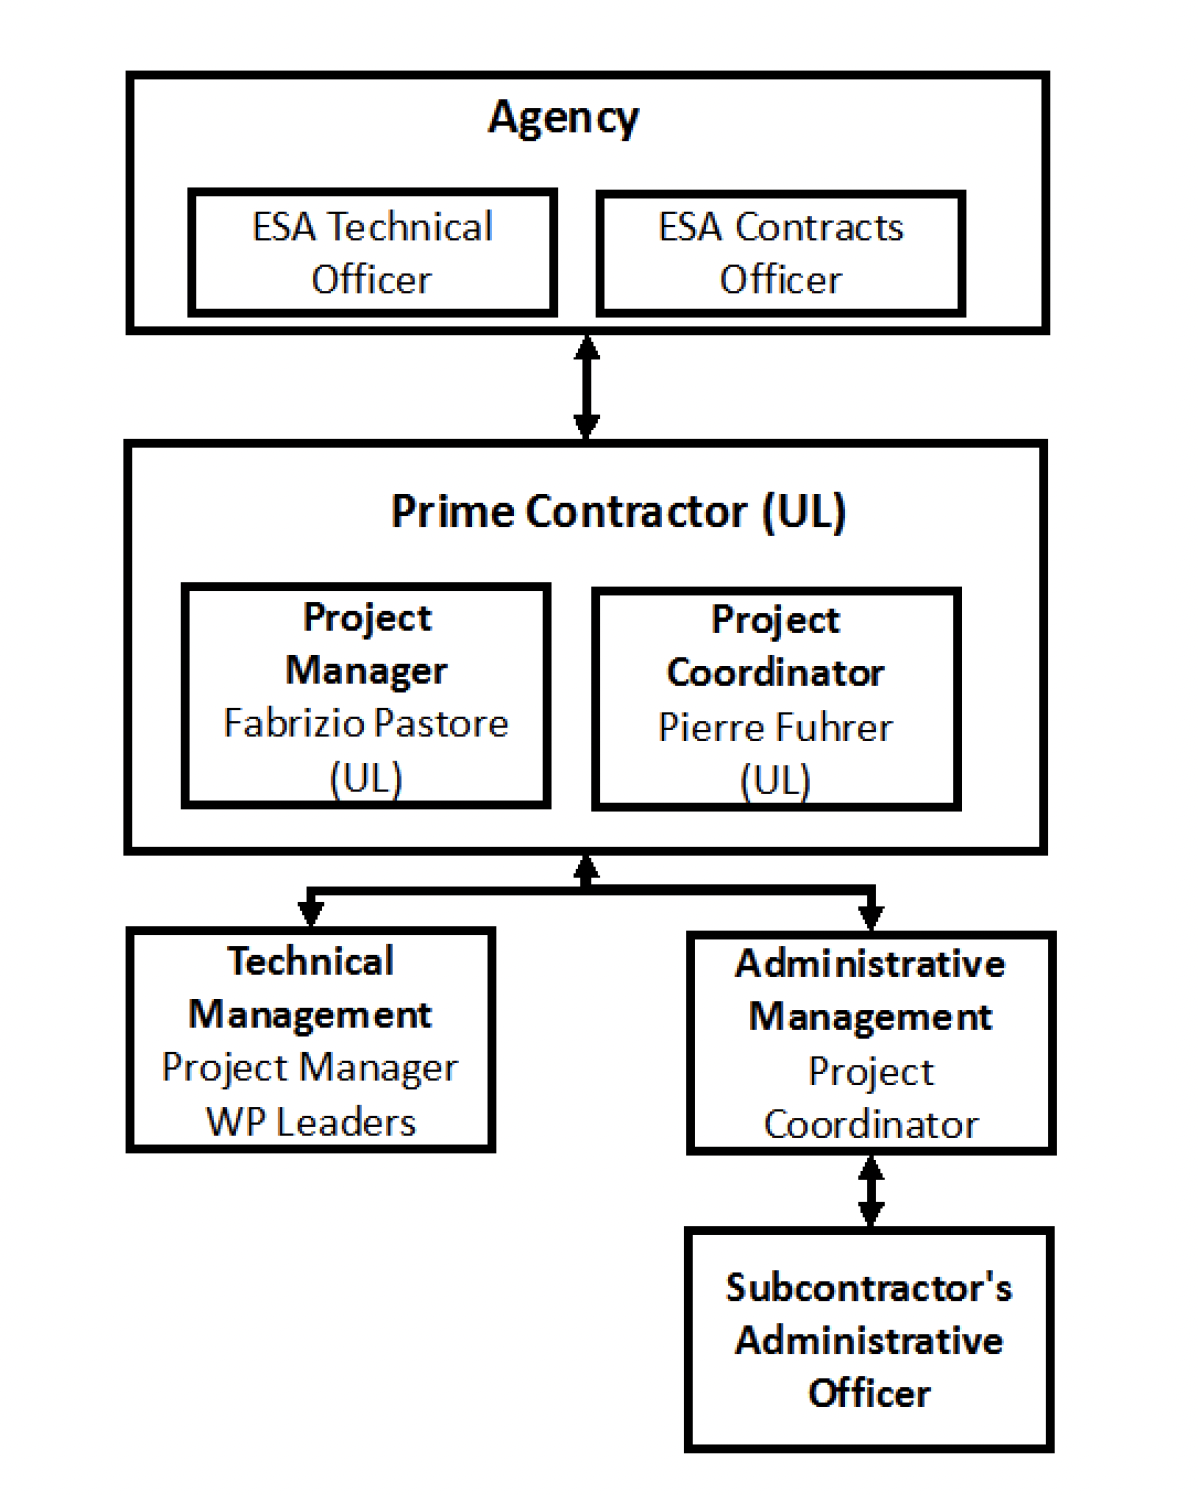
\includegraphics[width=0.5\textwidth]{images/reporting_lines}
\end{figure}

\subsection{Management Objectives and Priorities}

The toolset will be developed by SnT following the defined milestones and validated in tandem with the project partners, with a focus on the following tasks:
\begin{enumerate}
  \item Analysis and survey of mutation testing
  \item Study of mutation testing applicability to space software
  \item Development of the mutation testing framework
  \item Evaluation of mutation testing process and methodology
definition
  \item Maintenance and improvement of the toolset.
\end{enumerate}


\clearpage


\subsection{Master Schedule}

Figure~\ref{fig:GANTT} shows the GANTT chart for the FAQAS project.
The keyword WPx.y and WPx.y.z is used to indicate a task that may have subtasks. The keywords TRx and TMx are used to indicate reviews and task milestones based on SoW. Reviews and milestones are depicted using red and green diamonds, respectively. The critical path is depicted in red and derives from the dependencies between the reviews and the beginning of the following tasks.

\begin{figure}[H]
\caption{GANTT chart for the activity.}
\label{fig:GANTT}
\centering
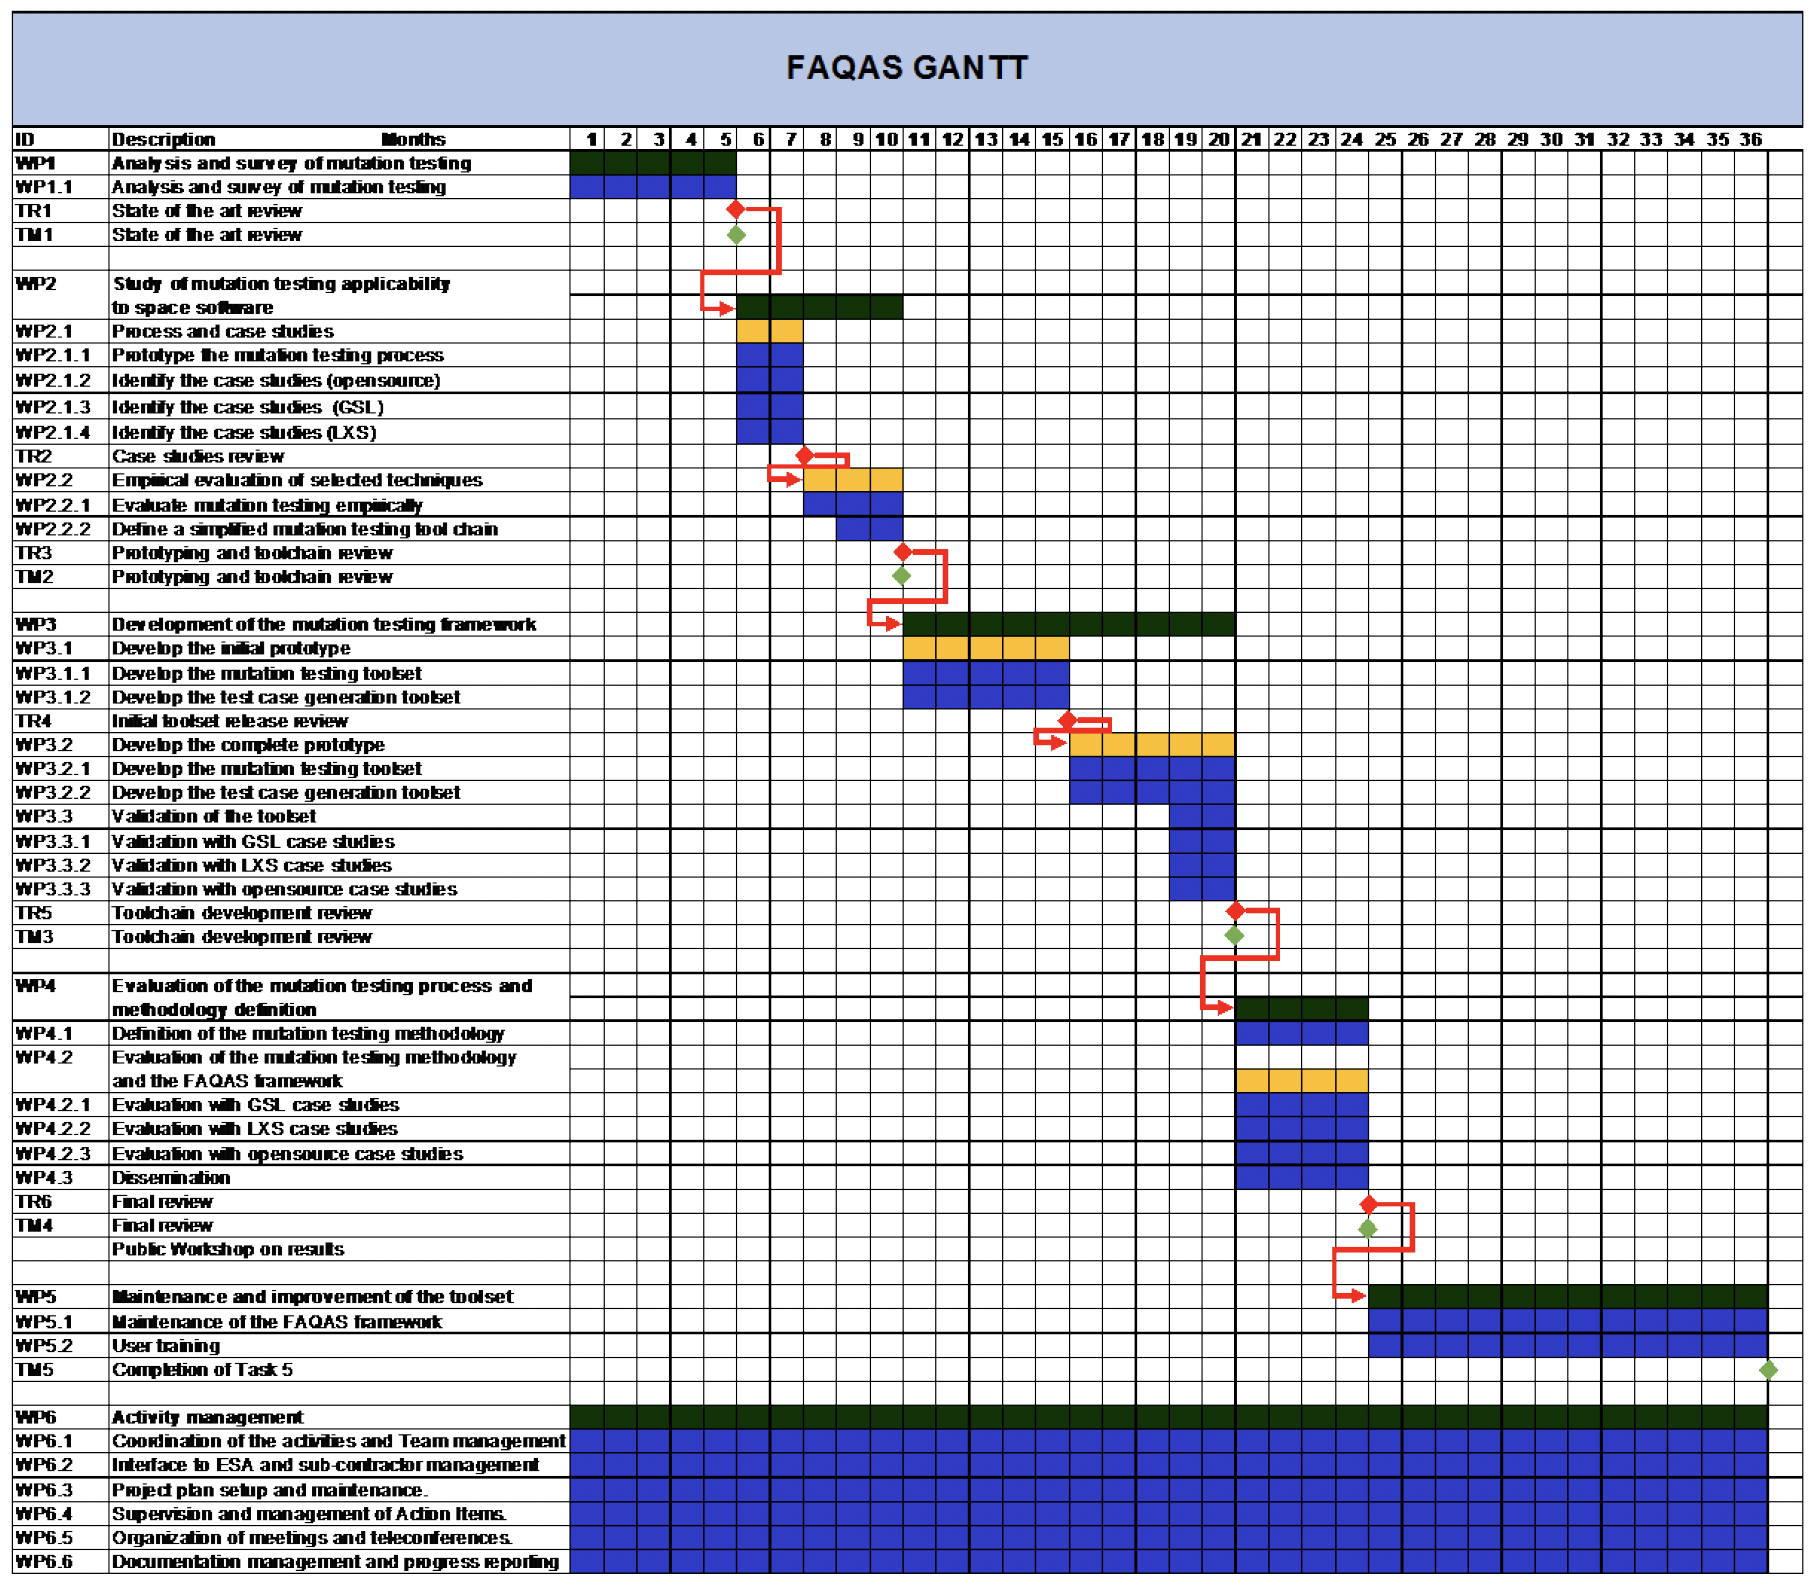
\includegraphics[width=\textwidth]{images/gantt}
\end{figure}

\clearpage

\subsection{Work Breakdown Structure}

Figure~\ref{fig:work_breakdown} shows the work breakdown structure. White boxes show work packages. Gray boxes show tasks within work packages. Boxes with thick lines correspond to tasks and work packages at the end of which a control milestone has been set. Work package and task identifiers match the ones used for the GANTT chart presented in the previous paragraph.

\begin{figure}[H]
\caption{Work breakdown structure.}
\label{fig:work_breakdown}
\centering
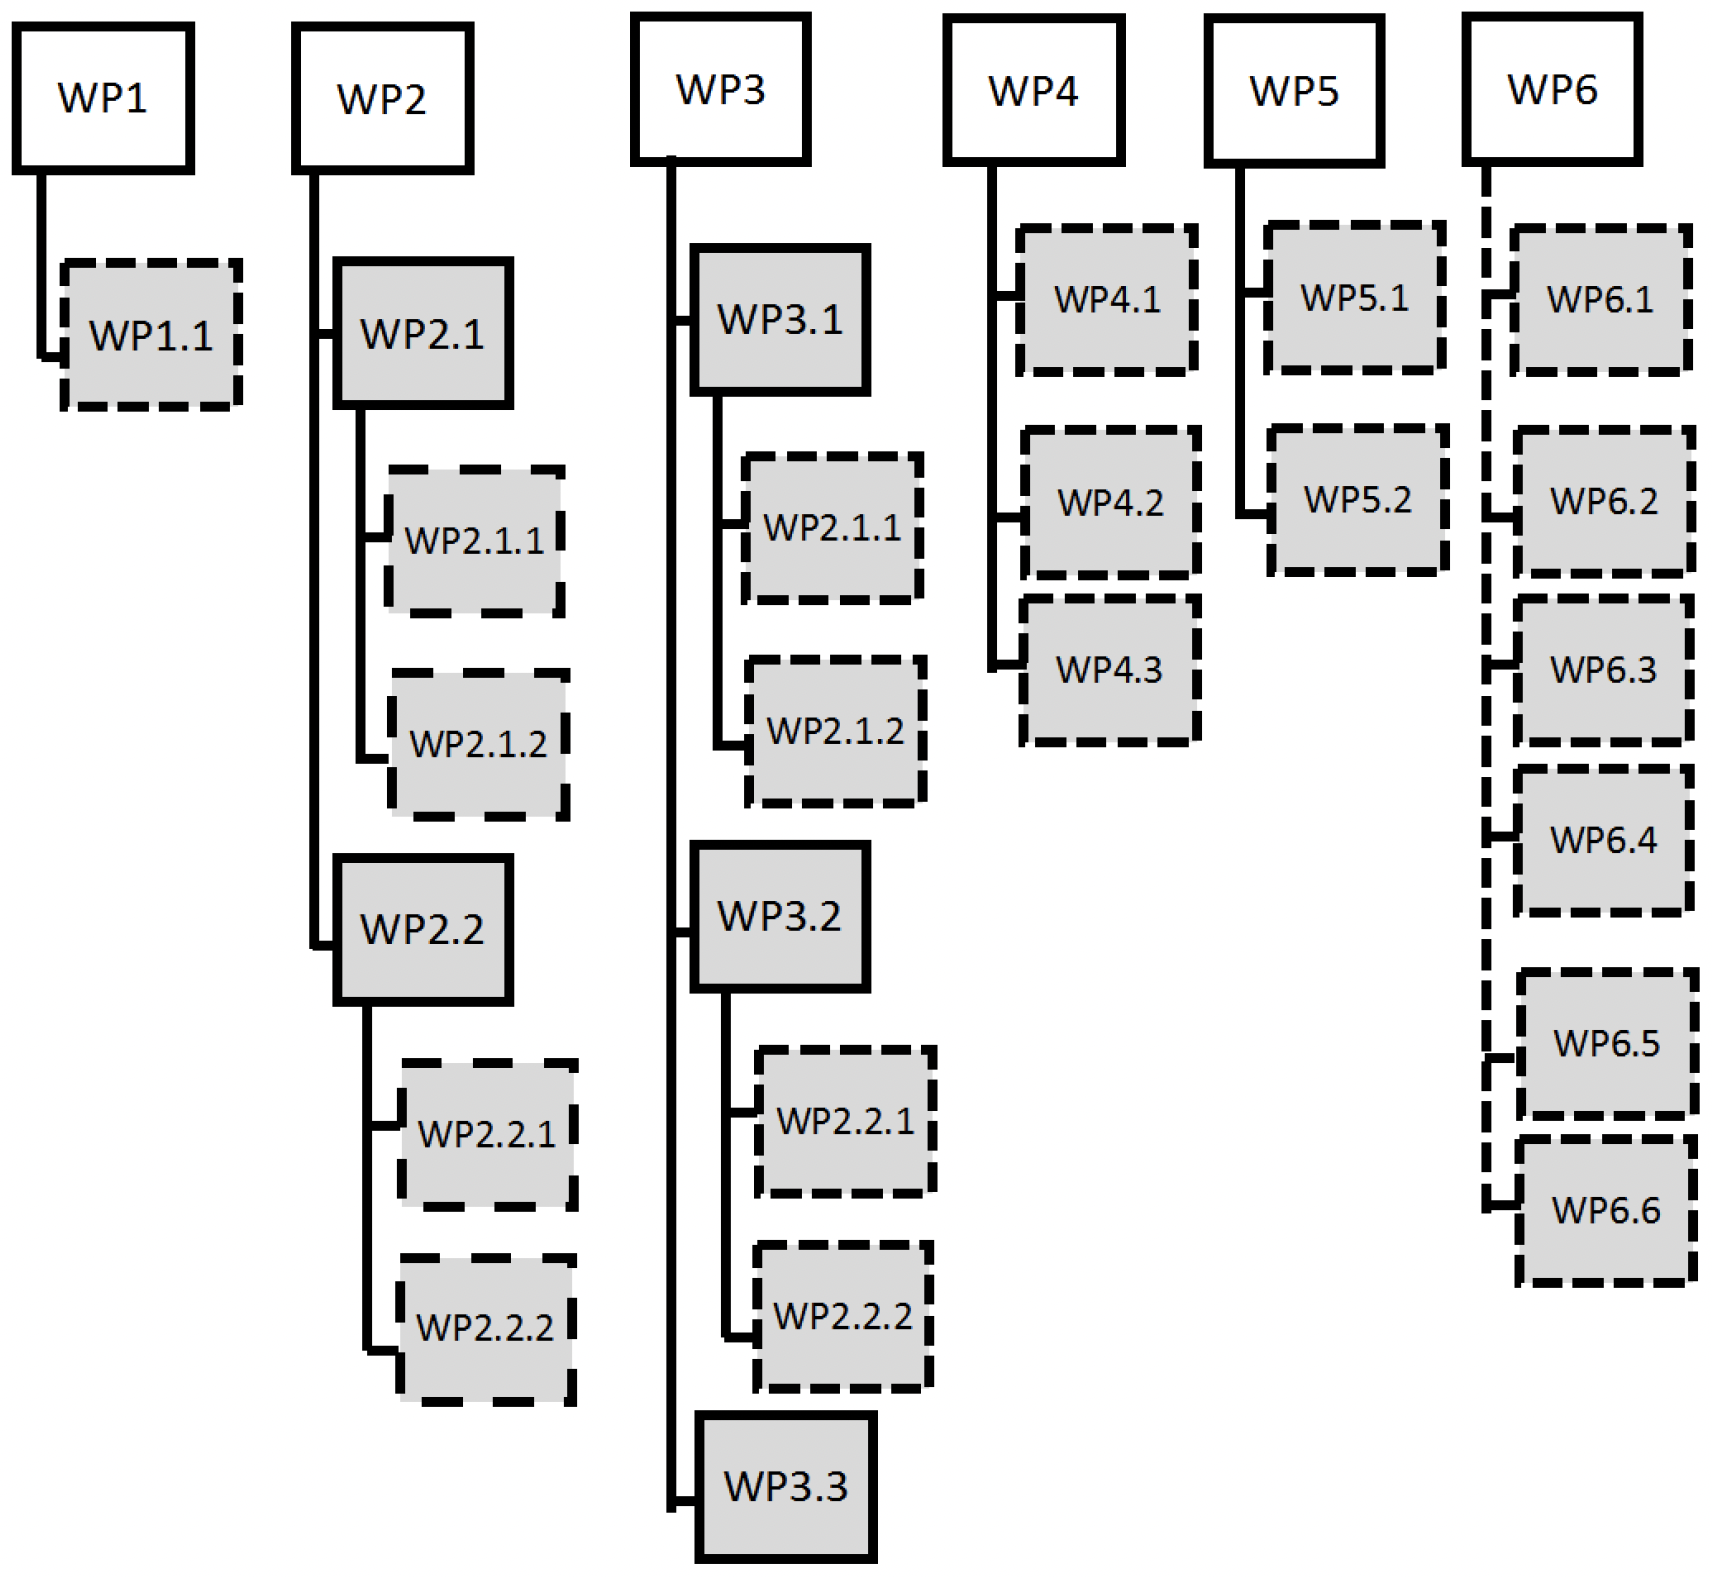
\includegraphics[width=0.5\textwidth]{images/work_breakdown}
\end{figure}

The description of the WP is presented in the following in tabular form.
Every WP is characterized by a list of activities with inputs and outputs consisting of both software and documentation items.

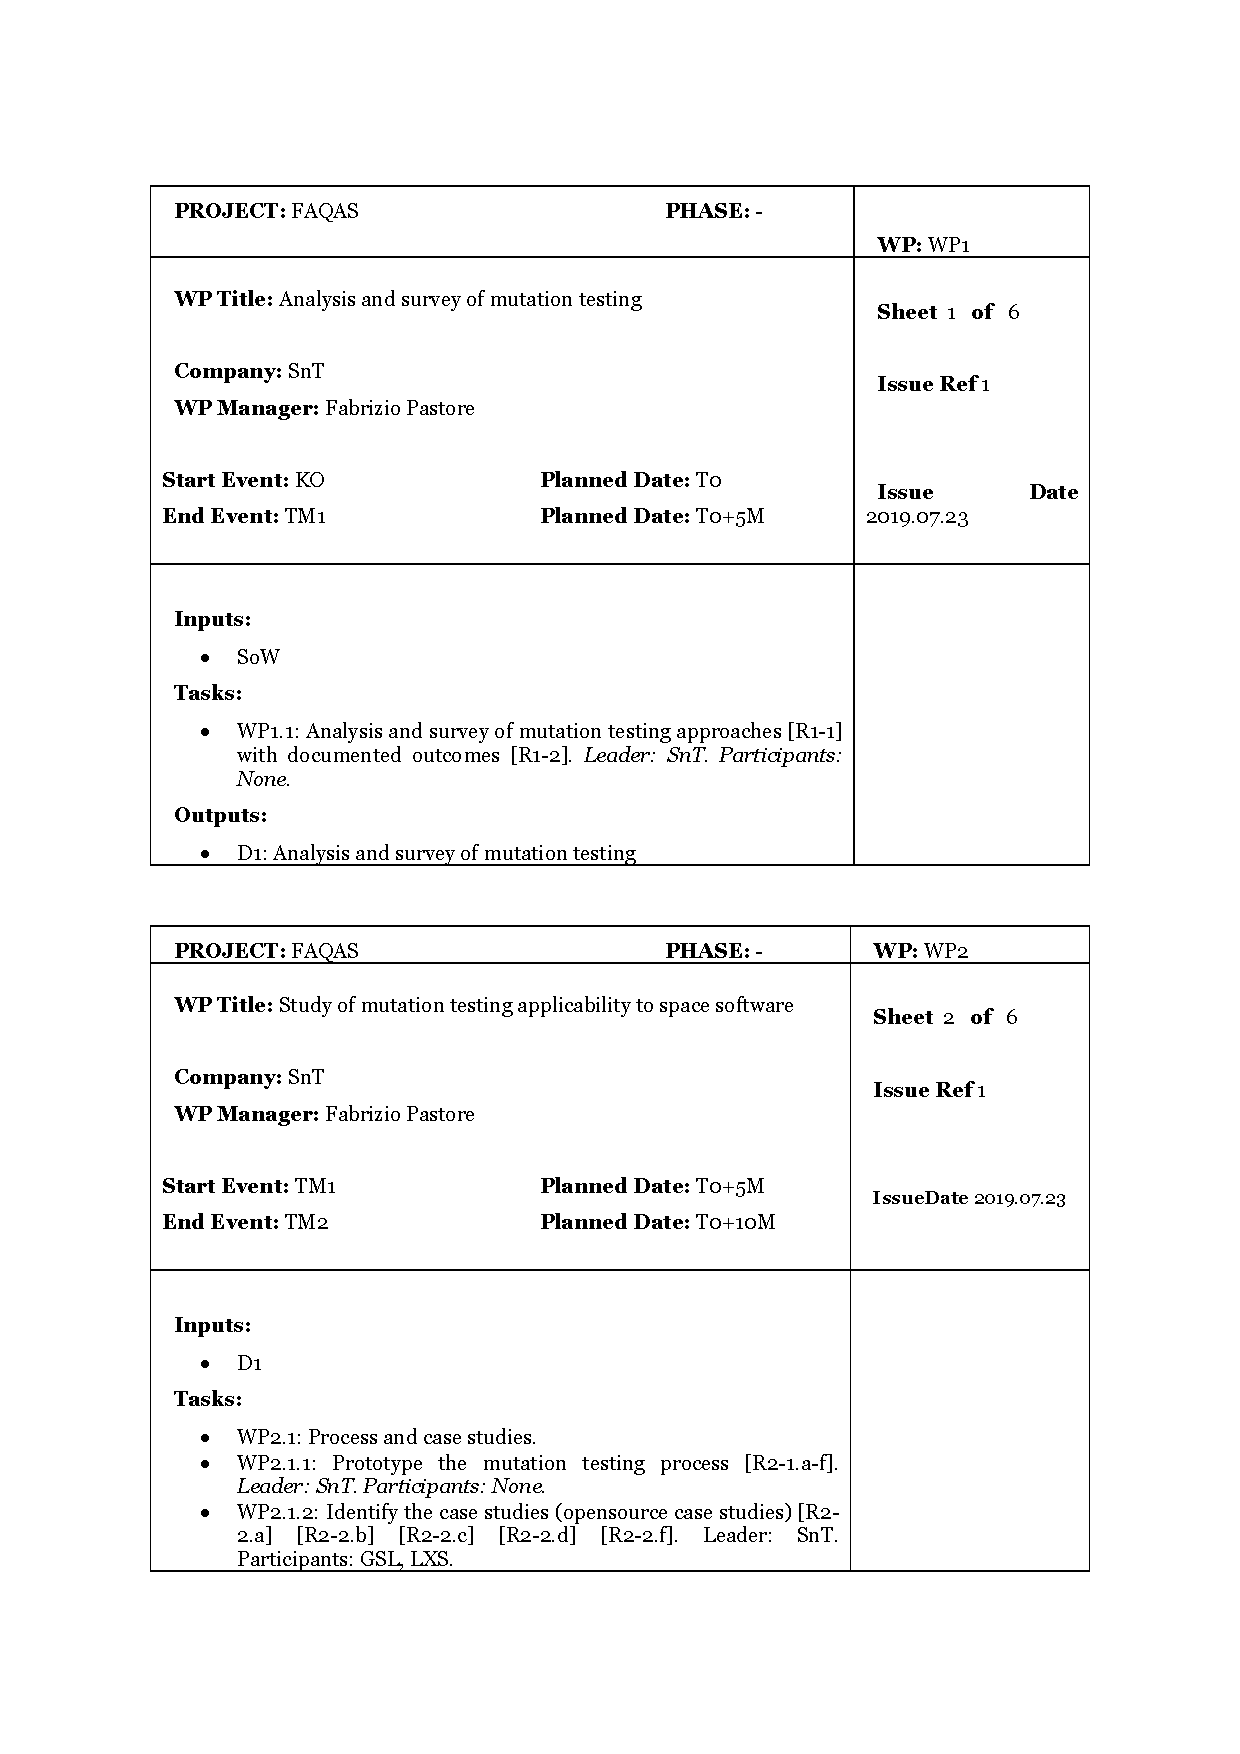
\includepdf[pages=-]{tables/work_packages.pdf}

\clearpage

\subsection{Monitoring and Controlling Mechanism}

The following monitoring and controlling mechanisms are in place:
\begin{itemize}
  \item Progress meetings,
  \item Progress reports,
  \item Reviews by partners.
\end{itemize}

\section{Software Development Approach}

The FAQAS framework is composed by the following software tools:
\begin{itemize}
  \item \MASS
  \item \DAMA
  \item \SEMUS
\end{itemize}

Every tool will be developed in accordance with the SSS and RB and validated through the use of unit testing and application to the selected case studies.
The project partners will also evaluate the toolset.

FAQAS has also lead to the definition and the evaluation of the feasibility of the \DAMTE methodology. Validation results, however, have shown that underlying test generation technology does enable the implementation of a test automation tool.
